\documentclass[article]{jss}

\author{David Meyer\\Wirtschaftsuniversit\"at Wien \And 
        Fridolin Wild\\Wirtschaftsuniversit\"at Wien}

\title{\pkg{lsa}: an \proglang{R} Package for Latent Semantic Analysis}

\Plainauthor{David Meyer, Fridolin Wild} 
\Plaintitle{lsa: an R Package for Latent Semantic Analysis}
\Shorttitle{Latent Semantic Analysis}

\Abstract{
  Latent semantic analysis (LSA) has continuously stirred scientific interest
  since its invention in the early 1990ies. LSA combines the classical 
  vector space model -- well known in textmining -- with a 
  singular value decomposition (SVD), a two-mode factor analysis. Thereby, 
  bag-of-words representations of texts can be mapped into a modified vector
  space that is assumed to reflect semantic structure. LSA can be 
  applied for various purposes, e.g. to automatically evaluate free text 
  responses typical for educational assessments, to find relevant documents
  matching unstructured queries typical in an information retrieval setting,
  to build a thesaurus, or to automatically classify documents into 
  pre-existing categories.
 
  In this paper we describe the \pkg{lsa} package for the language and
  environment \proglang{R} and illustrate its proper use through 
  examples from the area of automated essay scoring. Besides the high-level
  core functionalities implementing the LSA process, the package includes
  several sets of supporting functions facilitating the LSA process in the 
  construction of document-term-matrices, in the application of text 
  preprocessing methods and weighting schemes, in the selection of the desired 
  number of factors, and calculation of similarities within the newly created, 
  latent semantic space.

}

\Keywords{lsa, latent semantic analysis, text technology, computer linguistics, \proglang{R}}
\Plainkeywords{lsa, latent semantic analysis, text technology, computer linguistics, R}

%% publication information
%% \Volume{13}
%% \Issue{9}
%% \Month{September}
%% \Year{2004}
%% \Submitdate{2004-09-29}
%% \Acceptdate{2004-09-29}

\Address{
  Fridolin Wild, David Meyer\\
  Institute for Information Systems and New Media\\
  Vienna University of Economics and Business Administration\\
  A-1090 Vienna, Austria\\
  E-mail: \email{firstname.surname@wu-wien.ac.at}
}

%% for those who use Sweave please include the following line (with % symbols):
%% need no \usepackage{Sweave.sty}

\begin{document}

\section[statistical technique]{Introduction}

  Derived from latent semantic indexing, LSA is intended to enable the 
  analysis of the semantic structure of texts. The basic idea behind LSA 
  is that the collocation of terms of a given document-term-space reflects 
  a higher-order -- latent semantic -- structure, which is obscured by 
  word usage (e.g. by synonyms or ambiguities). By using conceptual indices 
  that are derived statistically via a truncated singular value decomposition, 
  this variability problem is believed to be overcome, cf. \cite{landauer:1990}.
  
  more on LSA.
  
  In a typical LSA process, first a document-term matrix is constructed 
  from a given text base of \begin{math}n\end{math} documents containing 
  \begin{math}m\end{math} terms (see \begin{math}M\end{math} in figure~\ref{fig:process}). 
  This matrix \begin{math}M\end{math} of the size \begin{math}m \times n\end{math} 
  is then resolved by the singular value decomposition into the term vector 
  matrix \begin{math}T\end{math} (constituting the right singular vectors), 
  the document vector matrix \begin{math}D\end{math} (constituting the right 
  singular vectors) being both orthonormal and the diagonal matrix 
  \begin{math}S\end{math}. Multiplying the truncated matrices 
  \begin{math}T_{k}\end{math}, \begin{math}S_{k}\end{math} and 
  \begin{math}D_{k}\end{math} results in a new matrix \begin{math}M_{k}\end{math} 
  which is the least-squares best fit approximation of 
  \begin{math}M\end{math} with \begin{math}k\end{math} singular values.

  \begin{figure}
     \centering
     \label{fig:process}
     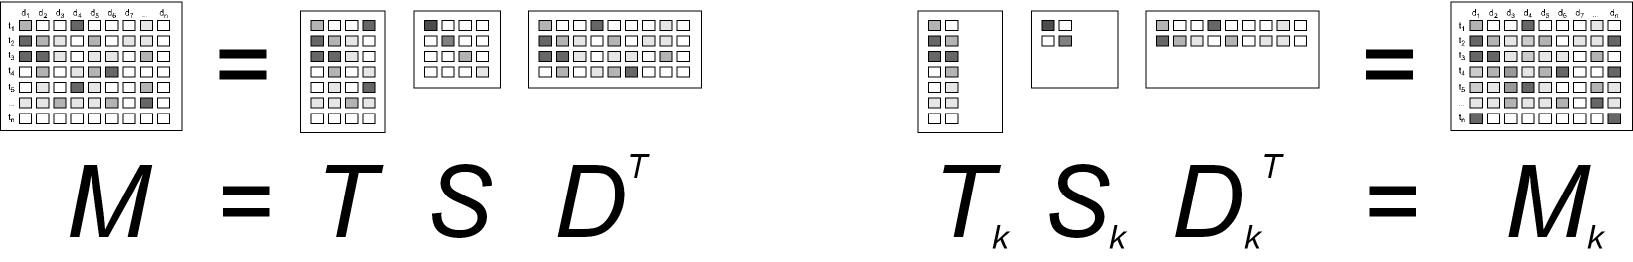
\includegraphics[width=140mm]{lsa_process.jpg}
     \caption{Singular Value Decomposition (original left, truncated right).}
  \end{figure}

\section[overview]{Latent Semantic Analysis}

Folding-In, Steps in the Process

\section[explaining code]{The \pkg{lsa} Package}

a section explaining the code

\section[examples]{Some Examples of Use}

a section with examples.
taken from essay scoring.

\section[conclusions]{Conclusions}

Future plans.

\section[acknowledgements]{Acknowledgements}

Christina Stahl, Gerald Stermsek, Gustaf Neumann, Yoseba Penya, Kurt Hornik, Stefan Sobernig.
Art Graeser, Max Louwerse, Roberto Turrin, Brian Ripley, Milos Kravcik, Goto...

\bibliography{lsa}

\end{document}
